\documentclass{standalone}
\usepackage{tikz}
\usetikzlibrary{3d}
\usetikzlibrary{patterns}
\usepackage{ifthen}


% Define colors
\definecolor{red}{RGB}{255,0,0}
\definecolor{green}{RGB}{0,255,0}
\definecolor{blue}{RGB}{0,0,255}
\definecolor{yellow}{RGB}{255,255,0}
\definecolor{white}{RGB}{255,255,255}
\definecolor{orange}{RGB}{255,165,0}

% Define the function to draw a single cubicle
\newcommand{\drawcubicle}[5][onn]{
  \ifthenelse{\equal{#1}{onn}}{
  \begin{scope}[shift={#2}]
    % Front face
    \begin{scope}[canvas is xy plane at z=0]
      \path[draw=black,#3] (0,0) rectangle (1,1);
    \end{scope}
    % Top face
    \begin{scope}[canvas is xz plane at y=1]
      \path[draw=black,#4] (0,0) rectangle (1,1);
    \end{scope}
    % Right face
    \begin{scope}[canvas is yz plane at x=1]
      \path[draw=black,#5] (0,0) rectangle (1,1);
    \end{scope}
  \end{scope}
}{}
}

\newcommand{\cubeCanvas}{
  % Draw the Rubik's Cube
  \foreach \x in {0,1,2} {
    \foreach \y in {0,1,2} {
      \foreach \z in {2,1,0} {
        \drawcubicle{(\x,\y,\z)}{draw=white}{draw=white}{draw=white}
      }
    }
  }
}


\pgfdeclarepatternformonly{upwards arrows}
  {\pgfpointorigin}{\pgfpoint{1cm}{0.3cm}}{\pgfpoint{1cm}{0.3cm}}
  {
  % Draw the triangles
  \pgfpathmoveto{\pgfpoint{0}{0}}
  \pgfpathlineto{\pgfpoint{0.25cm}{0}}
  \pgfpathlineto{\pgfpoint{0.5cm}{0.15cm}}
  \pgfpathlineto{\pgfpoint{0.75cm}{0}}
  \pgfpathlineto{\pgfpoint{1cm}{0}}
  \pgfpathlineto{\pgfpoint{0.5cm}{0.3cm}}
  \pgfpathlineto{\pgfpoint{0}{0}}
  \pgfpathclose
  \pgfusepath{fill}
}

\tikzset{front/.style={fill=red}}
\tikzset{top/.style={fill=white}}
\tikzset{right/.style={fill=blue}}
\tikzset{inner/.style={fill=gray!50!white,draw=black}}


\begin{document}

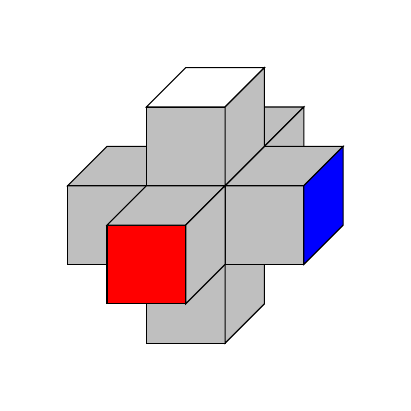
\begin{tikzpicture}[z={(0.5cm,0.5cm)}]
  \cubeCanvas
%%%% BOTTOM
\drawcubicle[off]{(0,0,2)}{inner}{inner}{inner} % 1
\drawcubicle[off]{(1,0,2)}{inner}{inner}{inner} %   2
\drawcubicle[off]{(2,0,2)}{inner}{inner}{right} %     3
\drawcubicle[off]{(0,0,1)}{inner}{inner}{inner} % 4
\drawcubicle[onn]{(1,0,1)}{inner}{inner}{inner} %   5
\drawcubicle[off]{(2,0,1)}{inner}{inner}{right} %     6
\drawcubicle[off]{(0,0,0)}{front}{inner}{inner} % 7
\drawcubicle[off]{(1,0,0)}{front}{inner}{inner} %   8
\drawcubicle[off]{(2,0,0)}{front}{inner}{right} %     9
%%
%%%% MIDDLE
\drawcubicle[off]{(0,1,2)}{inner}{inner}{inner} % 1
\drawcubicle[onn]{(1,1,2)}{inner}{inner}{inner} %   2
\drawcubicle[off]{(2,1,2)}{inner}{inner}{right} %     3
\drawcubicle[onn]{(0,1,1)}{inner}{inner}{inner} % 4
\drawcubicle[off]{(1,1,1)}{inner}{inner}{inner} %   5
\drawcubicle[onn]{(2,1,1)}{inner}{inner}{right} %     6
\drawcubicle[off]{(0,1,0)}{front}{inner}{inner} % 7
\drawcubicle[onn]{(1,1,0)}{front}{inner}{inner} %   8
\drawcubicle[off]{(2,1,0)}{front}{inner}{right} %     9
%%
%%%% TOP
\drawcubicle[off]{(0,2,2)}{inner}{top}{inner} % 1
\drawcubicle[off]{(1,2,2)}{inner}{top}{inner} %   2
\drawcubicle[off]{(2,2,2)}{inner}{top}{right} %     3
\drawcubicle[off]{(0,2,1)}{inner}{top}{inner} % 4
\drawcubicle[onn]{(1,2,1)}{inner}{top}{inner} %   5
\drawcubicle[off]{(2,2,1)}{inner}{top}{right} %     6
\drawcubicle[off]{(0,2,0)}{front}{top}{inner} % 7
\drawcubicle[off]{(1,2,0)}{front}{top}{inner} %   8
\drawcubicle[off]{(2,2,0)}{front}{top}{right} %     9
%%
\end{tikzpicture}

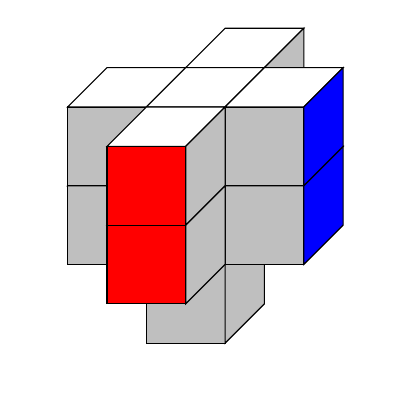
\begin{tikzpicture}[z={(0.5cm,0.5cm)}]
  \cubeCanvas
%%%% BOTTOM
\drawcubicle[off]{(0,0,2)}{inner}{inner}{inner} % 1
\drawcubicle[off]{(1,0,2)}{inner}{inner}{inner} %   2
\drawcubicle[off]{(2,0,2)}{inner}{inner}{right} %     3
\drawcubicle[off]{(0,0,1)}{inner}{inner}{inner} % 4
\drawcubicle[onn]{(1,0,1)}{inner}{inner}{inner} %   5
\drawcubicle[off]{(2,0,1)}{inner}{inner}{right} %     6
\drawcubicle[off]{(0,0,0)}{front}{inner}{inner} % 7
\drawcubicle[off]{(1,0,0)}{front}{inner}{inner} %   8
\drawcubicle[off]{(2,0,0)}{front}{inner}{right} %     9
%%
%%%% MIDDLE
\drawcubicle[off]{(0,1,2)}{inner}{inner}{inner} % 1
\drawcubicle[off]{(1,1,2)}{inner}{inner}{inner} %   2
\drawcubicle[off]{(2,1,2)}{inner}{inner}{right} %     3
\drawcubicle[onn]{(0,1,1)}{inner}{inner}{inner} % 4
\drawcubicle[onn]{(1,1,1)}{inner}{inner}{inner} %   5
\drawcubicle[onn]{(2,1,1)}{inner}{inner}{right} %     6
\drawcubicle[off]{(0,1,0)}{front}{inner}{inner} % 7
\drawcubicle[onn]{(1,1,0)}{front}{inner}{inner} %   8
\drawcubicle[off]{(2,1,0)}{front}{inner}{right} %     9
%%
%%%% TOP
\drawcubicle[off]{(0,2,2)}{inner}{top}{inner} % 1
\drawcubicle[onn]{(1,2,2)}{inner}{top}{inner} %   2
\drawcubicle[off]{(2,2,2)}{inner}{top}{right} %     3
\drawcubicle[onn]{(0,2,1)}{inner}{top}{inner} % 4
\drawcubicle[onn]{(1,2,1)}{inner}{top}{inner} %   5
\drawcubicle[onn]{(2,2,1)}{inner}{top}{right} %     6
\drawcubicle[off]{(0,2,0)}{front}{top}{inner} % 7
\drawcubicle[onn]{(1,2,0)}{front}{top}{inner} %   8
\drawcubicle[off]{(2,2,0)}{front}{top}{right} %     9
%%
\end{tikzpicture}

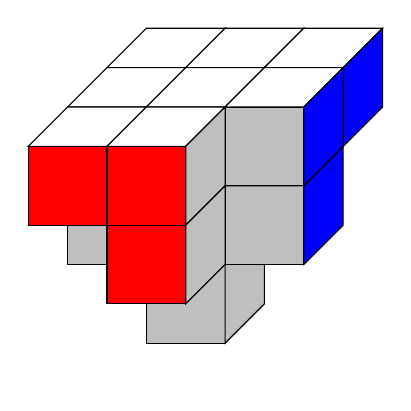
\begin{tikzpicture}[z={(0.5cm,0.5cm)}]
  \cubeCanvas
%%%% BOTTOM
\drawcubicle[off]{(0,0,2)}{inner}{inner}{inner} % 1
\drawcubicle[off]{(1,0,2)}{inner}{inner}{inner} %   2
\drawcubicle[off]{(2,0,2)}{inner}{inner}{right} %     3
\drawcubicle[off]{(0,0,1)}{inner}{inner}{inner} % 4
\drawcubicle[onn]{(1,0,1)}{inner}{inner}{inner} %   5
\drawcubicle[off]{(2,0,1)}{inner}{inner}{right} %     6
\drawcubicle[off]{(0,0,0)}{front}{inner}{inner} % 7
\drawcubicle[off]{(1,0,0)}{front}{inner}{inner} %   8
\drawcubicle[off]{(2,0,0)}{front}{inner}{right} %     9
%%
%%%% MIDDLE
\drawcubicle[off]{(0,1,2)}{inner}{inner}{inner} % 1
\drawcubicle[off]{(1,1,2)}{inner}{inner}{inner} %   2
\drawcubicle[off]{(2,1,2)}{inner}{inner}{right} %     3
\drawcubicle[onn]{(0,1,1)}{inner}{inner}{inner} % 4
\drawcubicle[onn]{(1,1,1)}{inner}{inner}{inner} %   5
\drawcubicle[onn]{(2,1,1)}{inner}{inner}{right} %     6
\drawcubicle[off]{(0,1,0)}{front}{inner}{inner} % 7
\drawcubicle[onn]{(1,1,0)}{front}{inner}{inner} %   8
\drawcubicle[off]{(2,1,0)}{front}{inner}{right} %     9
%%
%%%% TOP
\drawcubicle[onn]{(0,2,2)}{inner}{top}{inner} % 1
\drawcubicle[onn]{(1,2,2)}{inner}{top}{inner} %   2
\drawcubicle[onn]{(2,2,2)}{inner}{top}{right} %     3
\drawcubicle[onn]{(0,2,1)}{inner}{top}{inner} % 4
\drawcubicle[onn]{(1,2,1)}{inner}{top}{inner} %   5
\drawcubicle[onn]{(2,2,1)}{inner}{top}{right} %     6
\drawcubicle[onn]{(0,2,0)}{front}{top}{inner} % 7
\drawcubicle[onn]{(1,2,0)}{front}{top}{inner} %   8
\drawcubicle[off]{(2,2,0)}{front}{top}{right} %     9
%%
\end{tikzpicture}

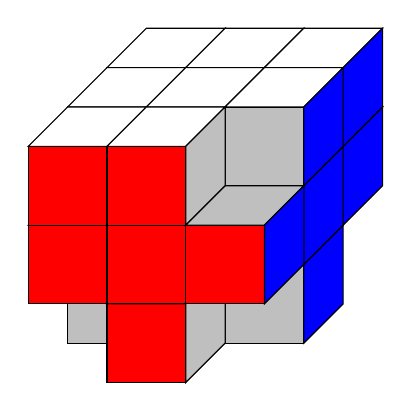
\begin{tikzpicture}[z={(0.5cm,0.5cm)}]
  \cubeCanvas
%%%% BOTTOM
\drawcubicle[off]{(0,0,2)}{inner}{inner}{inner} % 1
\drawcubicle[onn]{(1,0,2)}{inner}{inner}{inner} %   2
\drawcubicle[off]{(2,0,2)}{inner}{inner}{right} %     3
\drawcubicle[onn]{(0,0,1)}{inner}{inner}{inner} % 4
\drawcubicle[onn]{(1,0,1)}{inner}{inner}{inner} %   5
\drawcubicle[onn]{(2,0,1)}{inner}{inner}{right} %     6
\drawcubicle[off]{(0,0,0)}{front}{inner}{inner} % 7
\drawcubicle[onn]{(1,0,0)}{front}{inner}{inner} %   8
\drawcubicle[off]{(2,0,0)}{front}{inner}{right} %     9
%%
%%%% MIDDLE
\drawcubicle[onn]{(0,1,2)}{inner}{inner}{inner} % 1
\drawcubicle[onn]{(1,1,2)}{inner}{inner}{inner} %   2
\drawcubicle[onn]{(2,1,2)}{inner}{inner}{right} %     3
\drawcubicle[onn]{(0,1,1)}{inner}{inner}{inner} % 4
\drawcubicle[onn]{(1,1,1)}{inner}{inner}{inner} %   5
\drawcubicle[onn]{(2,1,1)}{inner}{inner}{right} %     6
\drawcubicle[onn]{(0,1,0)}{front}{inner}{inner} % 7
\drawcubicle[onn]{(1,1,0)}{front}{inner}{inner} %   8
\drawcubicle[onn]{(2,1,0)}{front}{inner}{right} %     9
%%
%%%% TOP
\drawcubicle[onn]{(0,2,2)}{inner}{top}{inner} % 1
\drawcubicle[onn]{(1,2,2)}{inner}{top}{inner} %   2
\drawcubicle[onn]{(2,2,2)}{inner}{top}{right} %     3
\drawcubicle[onn]{(0,2,1)}{inner}{top}{inner} % 4
\drawcubicle[onn]{(1,2,1)}{inner}{top}{inner} %   5
\drawcubicle[onn]{(2,2,1)}{inner}{top}{right} %     6
\drawcubicle[onn]{(0,2,0)}{front}{top}{inner} % 7
\drawcubicle[onn]{(1,2,0)}{front}{top}{inner} %   8
\drawcubicle[off]{(2,2,0)}{front}{top}{right} %     9
%%
\end{tikzpicture}

\end{document}
